\chapter{Comportamiento longitudinal}
\label{ch:longitudinal-model}

El comportamiento longitudinal es un problema de regresión sobre cómo ha de comportarse la aceleración del \ac{dvu} en función de la información existente alrededor. El perfil de aceleración para el conjunto general de conductores tanto del conjunto de test como del de entrenamiento se ilustran en la figura~\ref{fig:acceleration-profiles}.

\begin{figure}[!b]
	\centering
	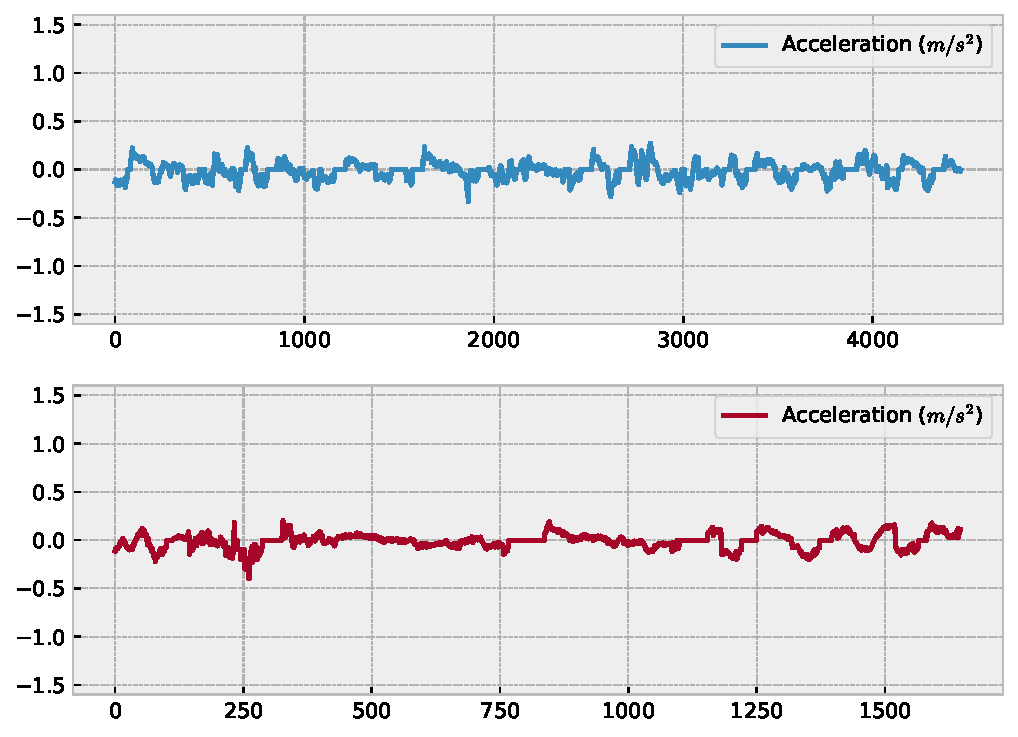
\includegraphics[width=\textwidth]{acceleration-profiles}
	\caption[Perfiles de aceleración a ajustar por los modelos. Conjuntos de entrenamiento y de test]{Perfiles de aceleración de los conjuntos de entrenamiento (arriba) y test(abajo).}
	\label{fig:acceleration-profiles}
\end{figure}

Por la naturaleza del problema se han seleccionado dos técnicas diferentes para el ajuste del modelo:

\begin{enumerate}
	\item \ac{mlp}. Al ser un problema de regresión, el uso de \acp{mlp} en el comportamiento longitudinal está justificado a ser considerados éstos aproximadores universales~\cite{hornik1991approximation}\sidenote{El \textit{Teorema de aproximación Universal} postula que un \ac{mlp} con al menos una capa oculta es capaz de aproximar cualquier función si dispone de suficientes neuronas en ésta.}
	\item \ac{fcs}. La formulación de este problema se ajusta muy bien al funcionamiento de estos modelos, donde en función de las entradas y de acuerdo a una serie de reglas, el controlador toma una decisión para la salida. Además, los \ac{fcs} tienen la ventaja de que se puede explicar cómo funcionan, cosa que no es posible para un \ac{mlp} con una o más capas ocultas.
\end{enumerate}

Ambos modelos se ajustarán con un procedimiento basado en el descenso del gradiente denominado ADAM~\cite{kingma2014adam}. Su aplicación a los \acp{mlp} es directa (después de todo es una técnica desarrollada dentro de área de las \gls{ann}), pero para \acp{fcs} es necesaria una representación que permita el uso de este método para su optimización. Esta representación es una de las aportaciones de esta tesis y se se explica en el apéndice \nameref{ch:fuzzy-controller-adjustment}.

\subsection{Descripción de los datasets}

Del conjunto de datos~\ref{tbl:main-variables} descrito en el capítulo~\nameref{ch:methodology} seleccionaremos aquellos indicadores de interés y generaremos un conjunto de entrenamiento y test para cada uno de los sujetos y un conjunto de entrenamiento y test para el total de conductores.

Dado que nuestros modelos se basan en un esquema \textit{feed-forward}, existe el inconveniente de que para ellos es imposible mantener una memoria del orden en el que se están sucediendo las entradas. Sin embargo, contamos con las derivadas de la posición respecto al líder y la velocidad (la aceleración y la velocidad al líder respectivamente), por lo consideramos que disponemos de información temporal suficiente para este problema en concreto.

El resultado de la generación de los datasets de entrenamiento y test para todos los sujetos se resume en la tabla~\ref{tbl:cf-datasets-description}

\begin{table}[t]
	\centering
	\caption[Descripción de los conjuntos de datos]{Descripción de los conjuntos de datos para el entrenamiento de los modelos.}
	\label{tbl:cf-datasets-description}
	\begin{tabular}{ccccc}
		\toprule
		& & & \multicolumn{2}{c}{Tamaño} \\
		& Entradas & Salidas & Entrenamiento & Test \\
		\midrule
		\rowcolor{black!20} $CF_{S_1}$ & $7$ & $1$ & $1089$ & $543$ \\
		$CF_{S_2}$ & $7$ & $1$ & $1313$ & $560$ \\
		\rowcolor{black!20} $CF_{S_3}$ & $7$ & $1$ & $2067$ & $668$ \\
		$CF_{S_A}$ & $7$ & $1$ & $4469$ & $1771$ \\
		\bottomrule
	\end{tabular}
\end{table}

\section{Modelo basado en \acrlongplsp{fcs}}

Se han realizado entrenamientos sobre arquitecturas con diferente número de particiones difusas en las variables. Las arquitecturas que se han considerado más relevantes (tras un proceso de ensayo y error con diferente número de particiones difusas) se describen en la tabla~\ref{tbl:cf-fcs-architectures}. 

\begin{table}
	\centering
	\small
	\caption[Resumen de las arquitecturas \ac{fcs} para el modelo longitudinal]{Resumen de las arquitecturas seleccionadas. La posición de cada número de la arquitectura indica a qué variable lingüística se refiere (\textit{Distancia al líder}, \textit{Distancia a siguiente TLS}, \textit{TLS en verde}, \textit{TLS en amarillo}, \textit{TLS en rojo}, \textit{Velocidad} y \textit{Velocidad de aproximación al líder} respectivamente). Su valor se corresponde al número de conjuntos difusos de la partición de cada una de ellas.}
	\label{tbl:cf-fcs-architectures}
	\begin{tabular}{cccccc}
		\toprule
		\multirow{2}{*}{} & \multirow{2}{*}{Arquitectura} & \multirow{2}{*}{Epochs} & \multicolumn{3}{c}{RMS}      \\ 
		& & & Entrenamiento & Validación & Test \\
		\midrule
		\rowcolor{black!20} $FCS_1$ & $2, 2, 2, 2, 2, 2, 2$ & $10^5$ & $0.059$ & $0.064$ & $0.062$  \\
		$FCS_2$ & $3, 3, 2, 2, 2, 3, 3$ & $10^5$ & $0.073$ & $0.079$ & $0.080$  \\
		\rowcolor{black!20} $FCS_3$ & $4, 3, 2, 2, 2, 3, 3$ & $10^5$ & $0.072$ & $0.078$ & $0.088$  \\
		$FCS_4$ & $5, 5, 2, 2, 2, 5, 5$ & $10^5$ & $0.063$ & $0.068$ & $0.109$  \\
		\bottomrule
	\end{tabular}
\end{table}

Todas las arquitecturas mantienen el número de conjuntos difusos asociados a las variables de estado del semáforo (verde, ámbar y rojo) a $2$. La razón es debido a que dicha variable sólo puede tomar dos valores, $0$ o $1$, y en la inicialización de sus respectivas particiones, estas variables ya toman dichos valores con un grado de pertenencia de $1$ en sus dominios.

Cada uno de los controladores se ha entrenado durante $250.000$ epochs. El proceso de entrenamiento seguido no ha sido el del ajuste de todas las variables a la vez. Esto se debe a que se ha comprobado que el ajuste de las variables que determinan las particiones difusas parece suceder órdenes de magnitud más rápido que el ajuste de los pesos asociados a las reglas.

\begin{figure}[t]
	\centering
	\subfloat[Distancia a líder]{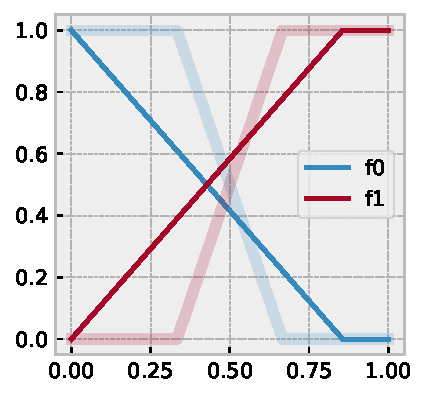
\includegraphics[width=.45\textwidth]{lm-fcs-best-architecture-leader-distance-variable-partition}}\qquad
	\subfloat[Distancia a siguiente semáforo]{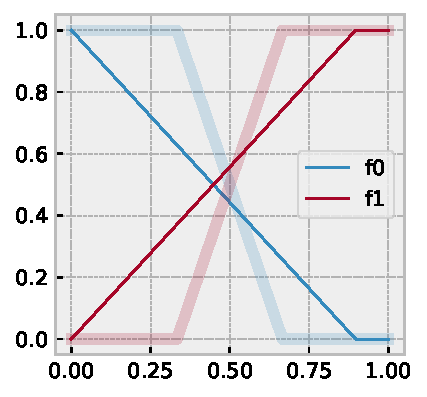
\includegraphics[width=.45\textwidth]{lm-fcs-best-architecture-next-tls-distance-variable-partition}}\qquad
	\subfloat[Velocidad]{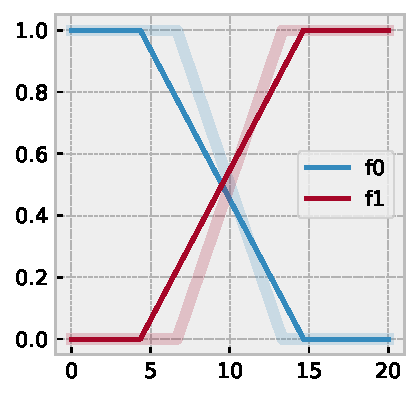
\includegraphics[width=.45\textwidth]{lm-fcs-best-architecture-speed-variable-partition}}\qquad
	\subfloat[Velocidad a líder]{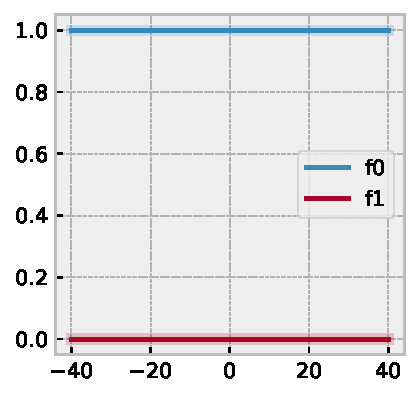
\includegraphics[width=.45\textwidth]{lm-fcs-best-architecture-speed-to-leader-variable-partition}}
	\caption[Particiones difusas después de la operación de ajuste en el modelo longitudinal basado en \ac{fcs}]{Particiones difusas despueés de la operación de ajuste en el modelo longitudinal basado en \ac{fcs}. Las funciones de pertenencia correspondientes al estado del semáforo no se incluyen ya que no se vieron modificadas en ningún entrenamiento. Después de todo, estas variables eran binarias, y las particiones difusas se inicializan de tal manera que dichos valores siempre alcanzan un valor de pertenencia $1$.}
	\label{fig:adjusted-fuzzy-partitions}
\end{figure}

\begin{figure}[!b]
	\centering
	\subfloat[]{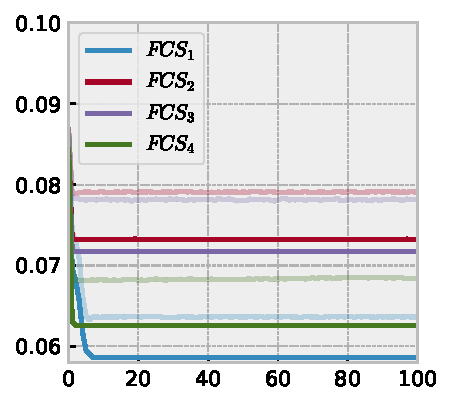
\includegraphics[width=.45\textwidth]{lm-fcs-rmse-all-training-and-validation-detail}}\qquad
	\subfloat[]{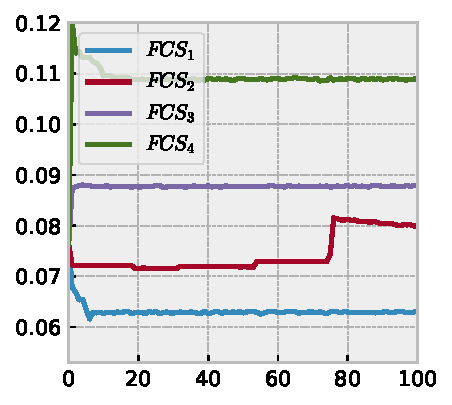
\includegraphics[width=.45\textwidth]{lm-fcs-rmse-all-test-detail}}
	\caption[Evolución del error durante el entrenamiento en las arquitecturas de \ac{fcs} para el modelo longitudinal]{Visión en detalle de la evolución del error en los conjuntos de entrenamiento y validación (izquierda) y de test (derecha). Para cada arquitectura, el color más transparente se corresponde al error en el conjunto de validación. El error de test se muestra debido a que nos ofrece puede ofrecer intuición de qué forma aprende la red, pero su evolución no se ha considerado para determinar las arquitecturas.}
	\label{fig:lm-fcs-rmse-all-comparisons}
\end{figure}

Por tanto, y para este problema en concreto, el entrenamiento se realiza iterativamente alternando conjuntos de epochs dedicados a las reglas y conjuntos de epochs dedicados a las variables de las reglas difusas.

En la Figura~\ref{fig:lm-fcs-rmse-all-comparisons} se puede observar la evolución en general y un detalle de la disminución del error durante el entrenamiento de los controladores. El error en test se ofrece a título informativo, y no ha sido usado para determinar las arquitecturas seleccionadas.

Se puede observar que la arquitectura $FCS_1$ es la que mejor error en test ha alcanzado. En las pruebas realizadas para el ajuste de controladores se ha observado además que los errores en entrenamiento y en test tienden a ser similares cuando los problemas son representables con un \ac{fcs}.

\begin{figure}[t]
	\centering
	\subfloat[]{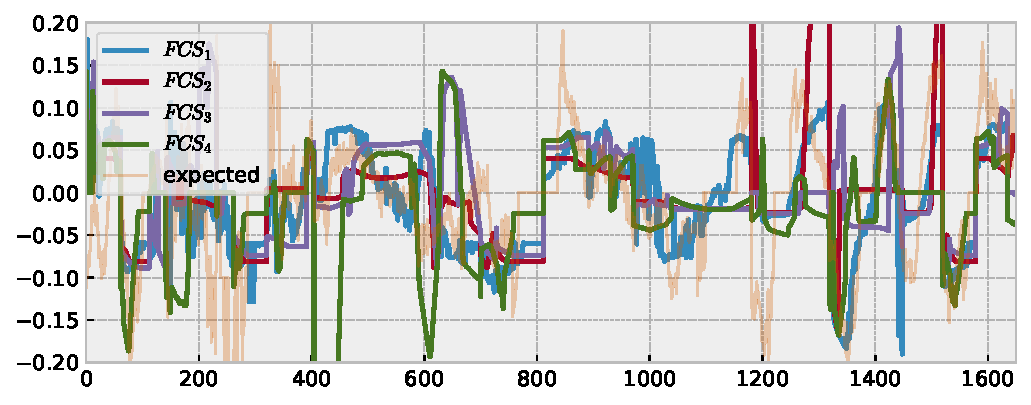
\includegraphics[width=\textwidth]{lm-fcs-outs-all-test-comparison}}\qquad
	\subfloat[]{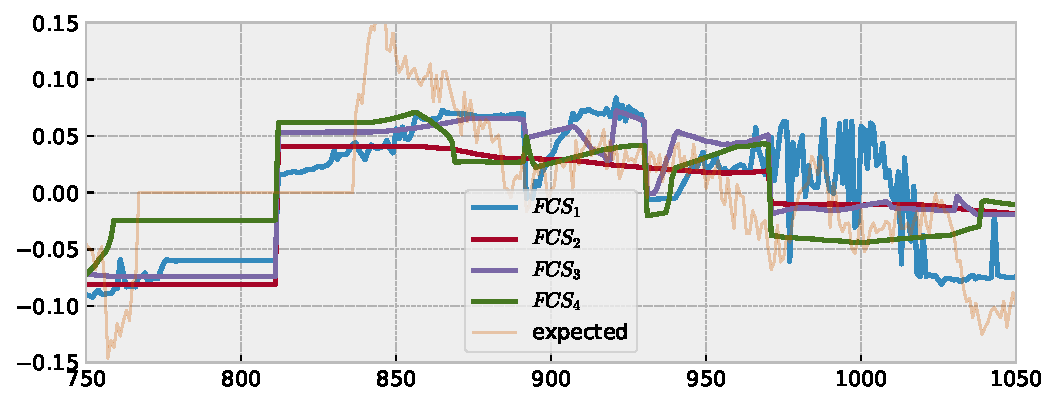
\includegraphics[width=\textwidth]{lm-fcs-outs-all-test-comparison-detail}}
	\caption[Comparación del perfil de aceleración real y el inferido por los modelos entrenados]{Comparación del perfil de aceleración real y el inferido por los modelos entrenados. En la visión general se puede observar, en transparente, el perfil real. A la derecha se amplía una pequeña sección del perfil para mostrar los diferentes ajustes de los modelos entrenados y cómo difieren del valor real.}
	\label{fig:fcs-test-comparisons}
\end{figure}

En lugar de eso se ha particionado el entrenamiento en secuencias sucesivas de entrenamiento de reglas y entrenamiento de particiones difusas. Concretamente, los $250.000$ epochs de entrenamiento se corresponden a $250$ iteraciones de $800$ epochs ajustando sólo las reglas seguidos de $200$ epochs ajustando las variables de las particiones difusas.

Empíricamente (y en este problema en concreto) se ha podido observar que el entrenamiento realizado de esta manera hace que el \ac{rmse} descienda más rápido en el mismo número de iteraciones.

En la Figura~\ref{fig:fcs-test-comparisons} se muestran los perfiles de la aceleración estimada por los controladores frente la aceleración real en cada momento. 

Tras el entrenamiento, el controlador difuso que menor error en test arroja es el $FCS_2$. Por tanto, éste será el modelo seleccionado para la comparativa final. Las funciones de pertenencia ajustadas se muestran en la Figura~\ref{fig:adjusted-fuzzy-partitions} contrastadas con las versiones de antes de comenzar el entrenamiento.

Las reglas, sin embargo, son muy numerosas para ser incluidas en el texto, ya que la mayoría de reglas posibles en el sistema tienen un peso asociado de más de $0.6$.

\section{Modelo basado en \acrlongplsp{mlp}}

Para determinar el modelo óptimo de \ac{mlp} en comportamiento longitudinal, se han realizado entrenamientos sobre arquitecturas con diferente cantidad de neuronas y capas ocultas. Las arquitecturas más ilustrativas de todas las probadas se resumen en la tabla~\ref{tbl:cf-mlp-architectures}.

\begin{table}
	\centering
	\caption[Resumen de las arquitecturas \ac{mlp} para el modelo longitudinal]{Resumen de las arquitecturas de \ac{mlp} para el modelo longitudinal. La posición de cada número de la topología indica el índice de la capa oculta y su valor el número de nodos (neuronas) que incluye dicha capa. Las arquitecturas seleccionadas en esta tabla son aquellas consideradas relevantes tras un proceso manual de ensayo y error.}
	\label{tbl:cf-mlp-architectures}
	\begin{tabular}{cccccc}
		\toprule
		\multirow{2}{*}{} & \multirow{2}{*}{Topología} & \multirow{2}{*}{Epochs} & \multicolumn{3}{c}{RMS} \\
		& & & Entrenamiento & Validación & Test \\
		\midrule
		\rowcolor{black!20} $MLP_1$ & $16$        & $10^5$ & $0.057$ & $0.057$ & $0.069$  \\
		$MLP_2$ & $8, 2$      & $10^5$ & $0.061$ & $0.061$ & $0.056$  \\
		\rowcolor{black!20} $MLP_3$ & $16, 8$     & $10^5$ & $0.051$ & $0.051$ & $0.060$  \\
		$MLP_4$ & $16, 16, 8$ & $10^5$ & $0.046$ & $0.046$ & $0.061$  \\
		\bottomrule
	\end{tabular}
\end{table}

\begin{figure}[!b]
	\centering
	\subfloat[Entrenamiento y validación]{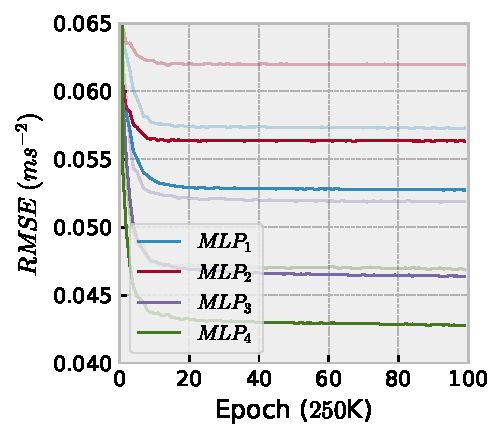
\includegraphics[width=.45\textwidth]{lm-mlp-rmse-all-training-and-validation-detail}}\qquad
	\subfloat[Test]{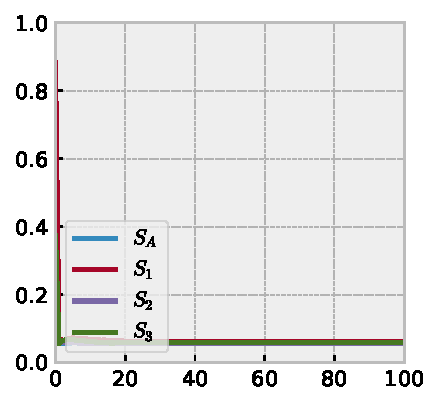
\includegraphics[width=.45\textwidth]{lm-mlp-rmse-all-test-detail}}
	\caption[Evolución del error durante el entrenamiento en las arquitecturas de \ac{mlp} para el modelo longitudinal]{Visión en detalle de la evolución del error en los conjuntos de entrenamiento y validación (izquierda) y de test (derecha). Para cada arquitectura, el color más transparente se corresponde al error en el conjunto de validación. El error de test se muestra debido a que nos ofrece puede ofrecer intuición de qué forma aprende la red, pero su evolución no se ha considerado para determinar las arquitecturas.}
	\label{fig:lm-mlp-rmse-all-comparisons}
\end{figure}

El modelo de neuronas de activación que se ha utilizado es de tipo tangente hiperbólica en todas las neuronas salvo en la última, que se ha utilizado una activación lineal en todas las neuronas salvo en la neurona de salida que se ha utilizado una activación lineal\sidenote{Se han utilizado también funciones de activación de tipo \ac{relu}, pero las tasas de error tras el entrenamiento eran notablemente más altas por lo que se ha optado al final por el uso de activación basada en tangente hiperbólica.}. Los pesos de la red han sido inicializados con una muestra aleatoria uniforme de valores reales en el intervalo $(-0.25, 0.25)$.

El error que se trata de minimizar es el error cuadrático medio entre los valores de aceleración del conjunto reales y los ajustados por el modelo. La Figura~\ref{fig:lm-mlp-rmse-all-comparisons} muestra la evolución de este error durante el proceso de entrenamiento. También se ilustra el error de test durante el mismo, aunque éste no se ha utilizado para decidir las arquitecturas y es simplemente informativo.

Estos errores se encuentran entre los \SI{0.05}{\metre\per\square\second} y los \SI{0.07}{\metre\per\square\second}, lo cual consideramos que es una aproximación aceptable. Una particularidad del problema ha sido la inestabilidad de los entrenamientos, esto es, la alta sensibilidad a los valores de inicialización de los parámetros. La intuición tras ver la evolución de los entrenamientos es que la función de error del problema tiene muchos mínimos locales o mesetas.

Al contrastar los errores de test, podemos determinar que la arquitectura que parece que mejor generaliza es la $MLP_2$ (arquitectura $7, 8, 2, 1$).

Una visión de detalle del ajuste de estas arquitecturas al conjunto de test se puede ver en la figura~\ref{fig:cf-mlp-test-comparisons}, donde se muestra el perfil de aceleración del conjunto de test y los perfiles de aceleración de las redes entrenadas.

A la vista de los resultados, y dado que las arquitecturas se ajustan razonablemente bien, es razonable elegir el modelo $MLP_2$ debido a que es el que aparentemente mejor generaliza los comportamientos del conjunto de conductores.

\begin{figure}[t]
	\centering
	\subfloat[Perfil completo]{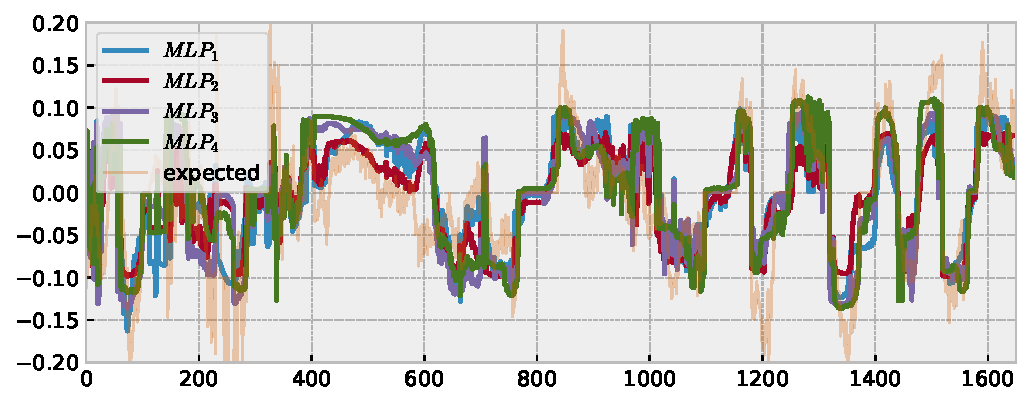
\includegraphics[width=\textwidth]{lm-mlp-outs-all-test-comparison}}\qquad
	\subfloat[Detalle]{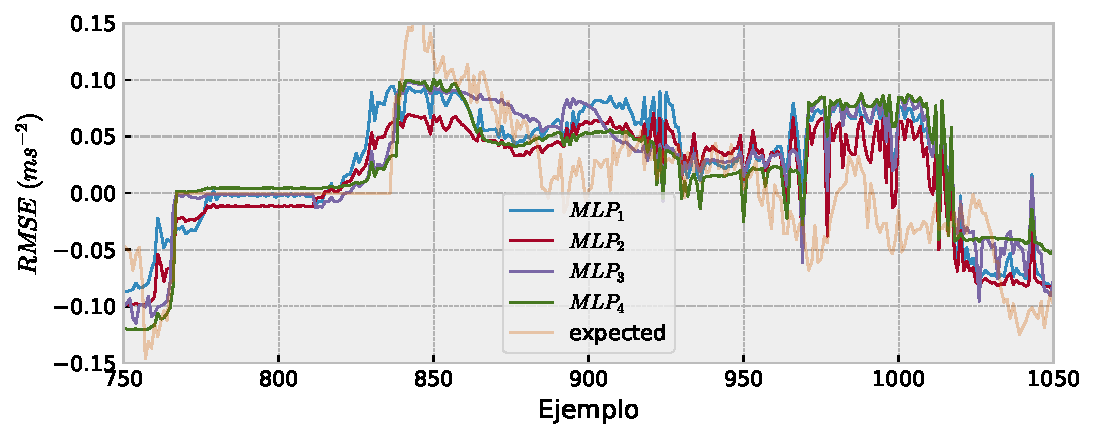
\includegraphics[width=\textwidth]{lm-mlp-outs-all-test-comparison-detail}}
	\caption[Comparación del perfil de aceleración real y el inferido por los modelos entrenados]{Comparación del perfil de aceleración real y el inferido por los modelos entrenados. En la visión general se puede observar, en transparente, el perfil real. A la derecha se amplía una pequeña sección del perfil para mostrar los diferentes ajustes de los modelos entrenados y cómo difieren del valor real.}
	\label{fig:cf-mlp-test-comparisons}
\end{figure}

\section{Comparación entre modelos}

Las mejores arquitecturas de ambos modelos han sido la $MLP_2$ para los \acp{mlp} y $FCS_x$ para los \acp{fcs}. Los errores y el perfil de aceleración para ambos modelos se muestran en la figura~\ref{fig:cf-comparison-between-best-mlp-and-fcs-architecture}.

\begin{figure}
	\centering
	\subfloat[Error en test]{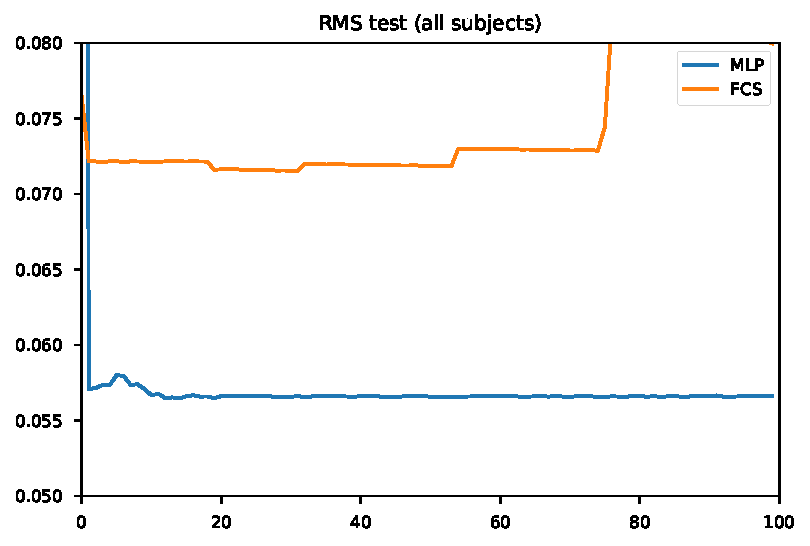
\includegraphics[width=.46\textwidth]{comparison-between-best-mlp-and-fcs-architecture-rms}}\qquad
	\subfloat[Perfil de aceleración]{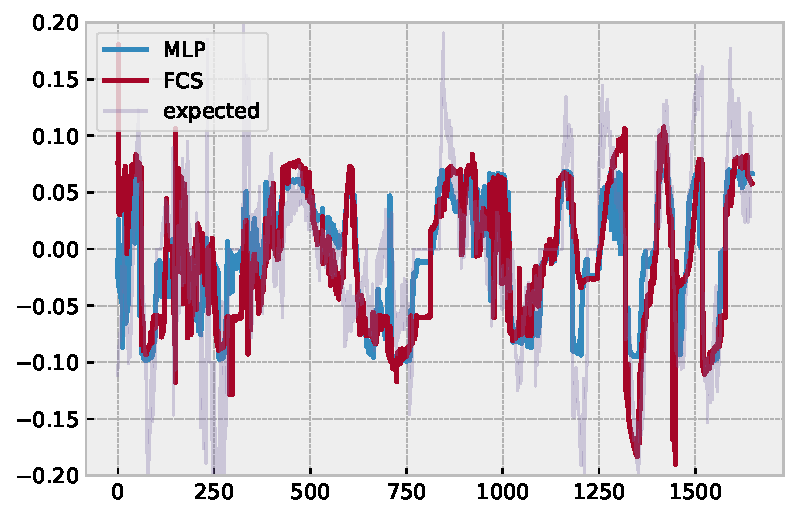
\includegraphics[width=.46\textwidth]{comparison-between-best-mlp-and-fcs-architecture-acceleration-profile}}
	\caption[Comparación entre los dos tipos de modelo longitudinal]{Comparación de la mejor arquitectura \ac{mlp} frente a la mejor arquitectura \ac{fcs}: (a) diferencia entre los errores cuadráticos medios de ambas arquitecturas y (b) perfiles de aceleración en el conjunto de test.}
	\label{fig:cf-comparison-between-best-mlp-and-fcs-architecture}
\end{figure}

Aunque el modelo basado en \ac{fcs} arroja un error bajo en test y parece que tiende a ajustarse al perfil de aceleración, parece que el problema es suficientemente complejo como para no poder representarse como un simple controlador difuso.

Además, el error arrojado por el \ac{mlp} es sustancialmente menor y, por tanto, la arquitectura elegida para el modelo longitudinal serála $MLP_2$.